\section{PBFT}
\subsection{背景}
BGP问题是BFT问题的一个特例:他假设所有节点对指挥官的身份形成了共识。实际的BFT问题里不一定有指挥官的存在,但拜占庭节点仍然存在。以下用$f$表示拜占庭节点的数量,用$n$表示总结点数量。解决问题的思路仍是沿用BGP问题的解法。

上一章我们提到了同步模型与异步模型的概念。这里指出,当我们研究区块链的共识算法的时候,鉴于区块链的大规模和去中心化,我们希望基于的都是异步模型的假设。现在的各项文献同步模型的研究已经不多。

然而异步环境共识不可避免的受限于FLP不可能定理:
\begin{theorem}
	当$f>0$,不存在一个确定的算法总能在异步网络环境下达成共识。
\end{theorem}
所以,各大著名的异步共识算法实际都做了各式各样的假设。如Ben-Or算法~\cite{ben1983another}引入随机性,即一定情况下需要节点各自通过掷硬币来选择决定,同时期望若干轮后所有诚实节点能掷出同样的结果。该算法仅能容忍$f<1/10n$的拜占庭节点,同时达到共识的期望轮数是指数级别。类似共享硬币~\cite{bracha1987asynchronous}的思路能够提升时间复杂度,但容错率仍然很低。

在正式介绍PBFT之前,我们这里简单介绍状态机复制,指的是一系列节点(初始状态相同)以相同的顺序执行一系列指令的问题。这个要求实际上比共识更强,因为像现在如比特币的共识是概率性的,即很难被扭转,但并不存在所谓的Finality状态,即完全一致性。而状态机复制需要保证完全的一致性。另外,如果一个算法能实现状态机复制(可能各文献说法会有不同,但这里我们默认状态机复制已经满足一致性),则可由该算法实现共识问题。

\textbf{为什么要用PBFT?}

最初,Paxos[]算法的提出解决了同步网络下没有拜占庭节点的状态机复制问题。然而,在区块链被提出之前,PBFT等一系列实现异步状态机复制的算法并没有受到重视。其原因是在传统的中心化系统中,对指令时序的一致性要求并没有那么强烈,往往会根据具体业务实现不同层面的一致性和安全性指标——一般而言,双机备份就足以满足大部分业务需求,同j时大部分情况下少量指令顺序的改变并不会对最终结果产生太大的影响。

区块链的诞生让尘封已久的BFT重建天日:由于区块链的大规模以及去中心化(意味着难回滚,不可篡改,冲突难以调和,需要备份的节点多)特性,人们需求一个状态机复制的强一致性保证。而其中最著名的算法就是PBFT,其全称为Practical Byzantine Fault Tolerance~\cite{castro1999practical},发表在1999年OSDI上。

\subsection{模型介绍}
传统的状态机复制算法或者依赖于同步网络环境的假设,或者在实际运行时间太慢。PBFT旨在提出能实现$1/3$异步拜占庭容忍的确定性协议,用于实现服务器副本按顺序执行一系列操作的问题。论文的假设是,在任何时刻$t$消息传输延迟$Delay(t)$不会无限制增长。这是一个非常弱的假设,在实际中通常是满足的。而这个假设的存在导致PBFT算法和FLP定理并不矛盾。

定义$\mathcal{R}=\{0,1,...,|\mathcal{R}|\}$,其中$|\mathcal{R}|=3f+1$。PBFT将所有服务器分为一个主节点和其他副本节点。每个节点在他的视角看到的信息称为一个view,每个节点的view允许不同。一般而言,主节点由$p=v mod R$决定,其中$v$表示view的轮数,在算法里会不断更新。

大致而言,PBFT算法执行包涵下面4个步骤:
\begin{itemize}
	\item 客户端向主节点发送一个操作请求
    \item 主节点向所有副本节点广播这个请求
    \item 所有副本节点执行这个请求,并且给客户端发送一个带执行结果的回复(reply)
    \item 当客户端收到至少$f+1$个相同的回复时,即得到该操作请求的执行结果。
\end{itemize}

客户端等待f+1个从不同副本节点得到的同样响应,同时需要保证签名正确,并且具有同样的时间戳t和执行结果r。这样客户端才能把r作为正确的执行结果,因为失效的副本节点不超过f个,所以f+1个replicas的一致响应必定能够保证结果是正确有效的。

如果客户端没有在有限时间内收到回复,请求将向所有副本节点进行广播。如果请求已经在副本节点处理过了,副本节点就向客户端重发一遍执行结果。如果请求没有在副本节点处理过,该副本节点将把请求转发给主节点。如果主节点没有将该请求进行广播,那么就有认为主节点失效,如果有足够多的副本节点认为主节点失效,则会触发一次view change,即主节点轮换。

对于一个客户端而言,在他的视角内仅仅的是简单的发送一个请求以及接受多个回复的过程。所以PBFT的核心部分在于服务器节点之间的交互,被分为三个部分:\emph{pre-prepare, prepare, commit}。见~\reffig{fig:PBFT1}。
\begin{figure}
	\centering
	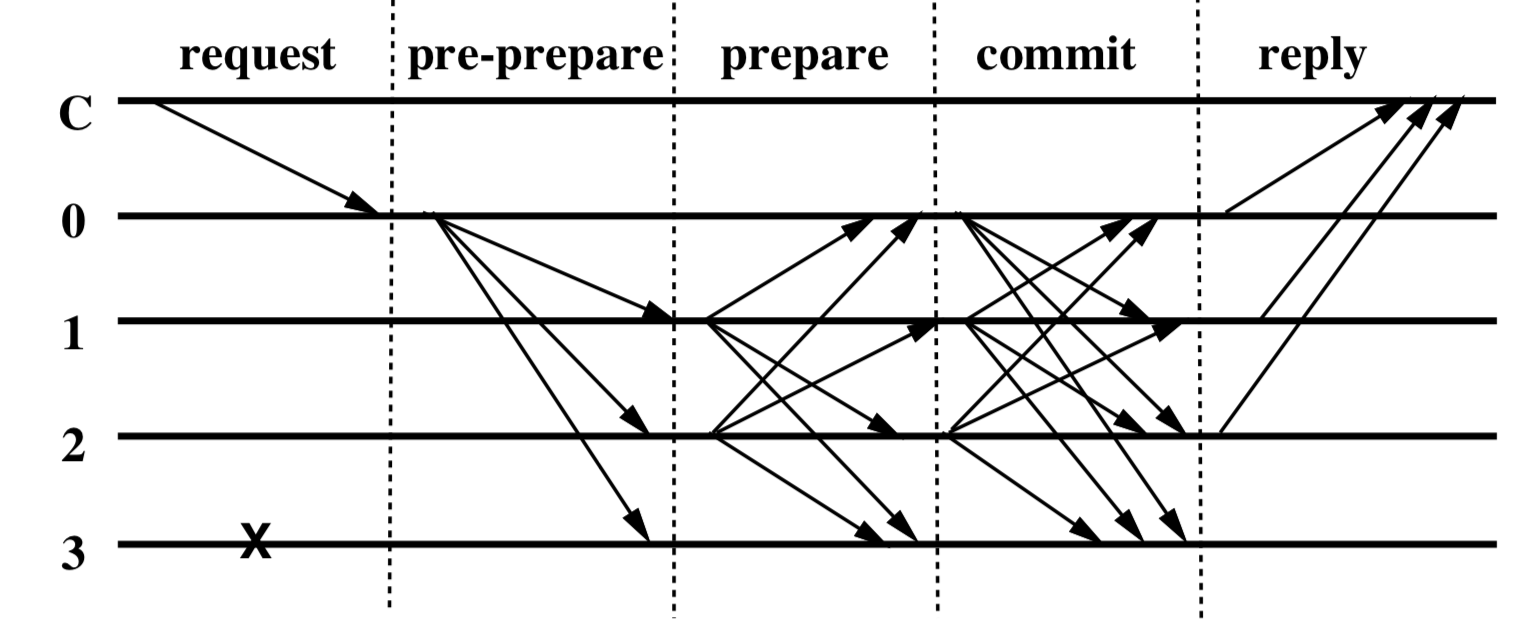
\includegraphics[width=1\textwidth]{../common/PBFT_1.png}
	\caption{PBFT流程} 
	\label{fig:PBFT1}
\end{figure}
\begin{itemize}
	\item \emph{pre-prepare}: 主节点分配一个序列号$n$给收到的请求($m$),然后向所有子节点广播pre-prepare消息$+m$,同时将请求消息$m$写入消息日志。消息的格式为$<PRE-PREPARE,v,n,d>_{\sigma_p},m>$,这里$v$是视图编号,$m$是客户端发送的请求消息,$d$是请求消息$m$的摘要(摘要在文章中的意思即哈希值$D(m)$,密码学上难以做逆运算),$\sigma_p$为主节点$p$的签名,$n$是消息的序号,必须在$h$和$H$之间(称为水线(watermark)限制这样可以防止拜占庭节点使用很大的$n$消耗序号空间)。注意为减少传输开销,此处客户端的原始请求并没有包括在pre-prepare消息内。副本节点只会接受格式,签名,view,水线限制均满足的pre-prepare消息。
	
    \item \emph{prepare}: 一旦副本节点接受了$<PRE-PREPARE,v,n,d>,m>$,则进入prepare阶段,同时。该节点向所有副本节点发送准备消息$<PREPARE,v,n,d,i>_{\sigma_i	}$,并且将两者写入自己的消息日志。定义$prepared(m,v,n,i)$为真当且仅当副本节点$i$已将下列消息写入日志:消息$m$,针对$m$且view为$v$且序号为$n$的pre-prepare消息,$2f$个从不同副本节点发来的与pre-prepare消息匹配的prepare消息。预准备阶段和准备阶段确保所有正常节点对同一个视图中的请求序号达成一致。预准备阶段和准备阶段确保所有正常节点对同一个视图中的请求序号达成一致,即$prepared(m,v,n,i)$和$prepared(m',v,n,j)$不能同时为真(若$m\neq m'$)。
    
    \item 当$prepared(m,v,n,i)$为真的时候,副本节点$i$将$<COMMIT,v,n,D(m),i>$向其他replicas广播,于是就进入了确认阶段。此阶段定义了两个函数,$committed(m,v,n)$为真的条件为:存在$f+1$个正常副本节点集合中使得其中所有副本节点$i$的$prepared(m,v,n,i)$为真。$committed-local(m,v,n,i)$为真的条件为:$prepared(m,v,n,i)$为真,并且$i$已经接受了$2f+1$个commits(包括自身在内)与pre-prepare消息一致。commit与pre-prepare消息一致的条件是具有相同的视图编号、消息序号和消息摘要。对某个正常节点$i$来说,如果$committed-local(m,v,n,i)$为真则$committed(m,v,n)$	也为真。这个不变式和视图变更协议保证了所有正常节点对本地确认的请求的序号达成一致,即使这些请求在每个节点的确认处于不同的视图。更进一步地讲,这个不变式保证了任何正常节点的本地确认最终会确认至少$f+1$个的正常副本。
\end{itemize}
视图变更协议:	所谓视图变更即将$v$加1,进而更换主节点。视图变更协议在主节点失效的时候仍然保证系统的活性。视图变更可以由超时触发,以防止副本节点无期限地等待请求的执行。

如果仅仅是这样,这个拜占庭容错在异步系统中是无效的。因为这个算法会在延迟超过阈值$t$的时候失效,而异步系统的定义就是找不到这样一个阈值$t$。PBFT采用的方法是:在$p=1$的时候,把阈值设为$t_1$,然后如果超时,则增加这个阈值。这样保证无论这个系统的延迟有多大,\emph{只要延迟不会无限增长},PBFT都能保证最终达成共识。

论文最后证明PBFT的安全性(safety)与活性(liveness),并进行了实验测试性能。这里不详细介绍,有兴趣的读者可以参阅全文。

\subsection{思考}
PBFT的好处是能够实现异步一致性,并且已经被大量区块链主要是联盟链项目所采用。其缺点在于共识的达成用到了长达三轮的消息传播,相对较长。在节点数量较少的情况下仍不失为一种最优的选择。
